\chapter{The Future of Epithelial Modeling}
\label{chap:advances}

We have thusfar explored the nature of epithelial tissue, discussed the variety of models that are currently in use, and thoroughly examined the \emph{Epithelium} implementation the Honda-Nagai Model. In this chapter, we will discuss some ideas for future epithelial tissue models. 

\begin{figure}[hb]
\centering
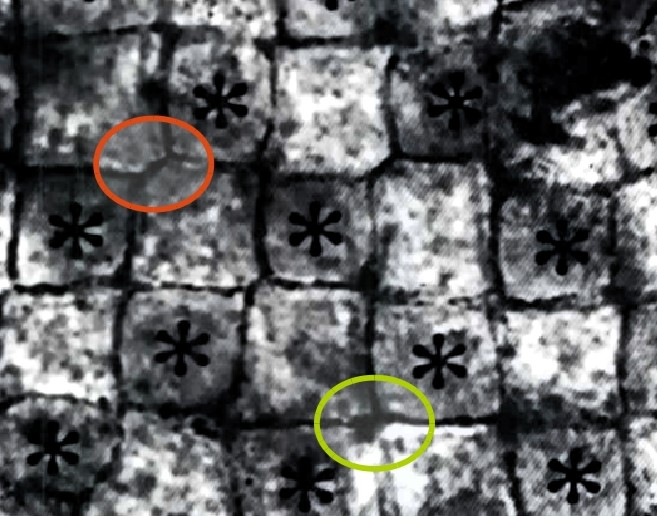
\includegraphics[width=0.5\textwidth]{../diagrams/checkers.jpg}
\caption{\textbf{Square Cells in Quail Epithelium. Image courtesy of~\cite{Checkers}.}}
\label{fig:quail}
\end{figure}

\section{Rosette Models}
We have discussed the standard topology of epithelial tissue in great detail, but now we will explore a potential model with much different connectivity. Most models of epithelial tissue exclusively support vertices of degree three, but there is at least one tissue for which this topology may not be accurate. Figure~\ref{fig:quail} is taken from a paper by H. Yamanaka and H. Honda~\cite{Checkers} in which they model the dynamics of Japanese quail epithelium using exclusively degree three vertices. The fact is, however, that Figure~\ref{fig:quail} lends itself equally to interpretation as a mesh of degree four vertices or degree three vertices. It seems intuitively unlikely that the epithelial tissue of Japanese quails be the only tissue with this appearance, and a reasonable research idea is to find what other tissues have this property, and then subject meshes of this type to Honda-Nagai forces to see if the mesh remains a stable quadrilateral mesh as in nature. This type of experimentation could help resolve whether or not the Honda-Nagai Model is a good model for all types of tissue, or if it is strictly suited to tissues with predominantly six sided cells in equilibrium. In its current incarnation \emph{Epithelium} can only handle three cells meeting at a vertex, but more energy could be invested to make it handle different connectivities.

\section{A New Potential, A New Force}
In the Honda-Nagai Model, a harmonic form is given for the potential energies due to area and perimeter deformations, the gradient of which givens a hookean form\footnote{Hooke's law says that $F=-k\Delta x$.} for the force applied to a node (for more details, refer to~\ref{sec:force}). The assumptions underlying a model can render even the most seemingly accurate model physically meaningless if the assumptions are proven to be incorrect, and for this reason we should be skeptical about the harmonic formulation. In the literature the $C(x-x_0)^2$ form for the potential energy is asserted without biological evidence that it is correct, or even reasonable. Furthermore, assuming that cells are indeed elastic, there is no reason to believe that their elasticity fits the linear stress-strain curves prescribed by the hookean model.

There is a large class of materials including rubber and various elastomers that are classified as neo-hookean hyperelastic materials because their stress-strain\footnote{The stress-strain curve is the curve showing the amount of deformation(strain) in a material due to the application of varying amounts of force (stress)} curves are only linear in a small region (See Figure~\ref{fig:rubber}). After this region, the elasticity of the material becomes much higher~\cite{Rubber, Rubber2}. Hyperelastic models have been applied to various tissues with impressive results as in~\cite{hyperbio, hyperbio2}, but have only been briefly discussed with respect to epithelial tissue, as in~\cite{epihyper, epihyper2}.

The ideas of hyperelasticity need to be explored in more detail, and the conditions under which the Honda-Nagai elastic model is plausible ought to be better examined.

\section{Improvements in Imaging}
Another recent development in epithelial tissue science is the ability to record high quality videos of epithelial tissue during morphogenesis. One of the most impressive examples to date is the work being done in the Kiehart lab at Duke University where they are recording the closing of the epithelial envelope of \emph{Drosophila} embryos~\cite{Sokolow}. Through their recordings they have produced very good fits for certain modeling parameters and have performed an interesting experiment in which they try to keep the envelope from closing, but it closes anyway due to some currently unknown mechanism. 

\begin{wrapfigure}{r}{0.5\textwidth}
  \begin{center}
    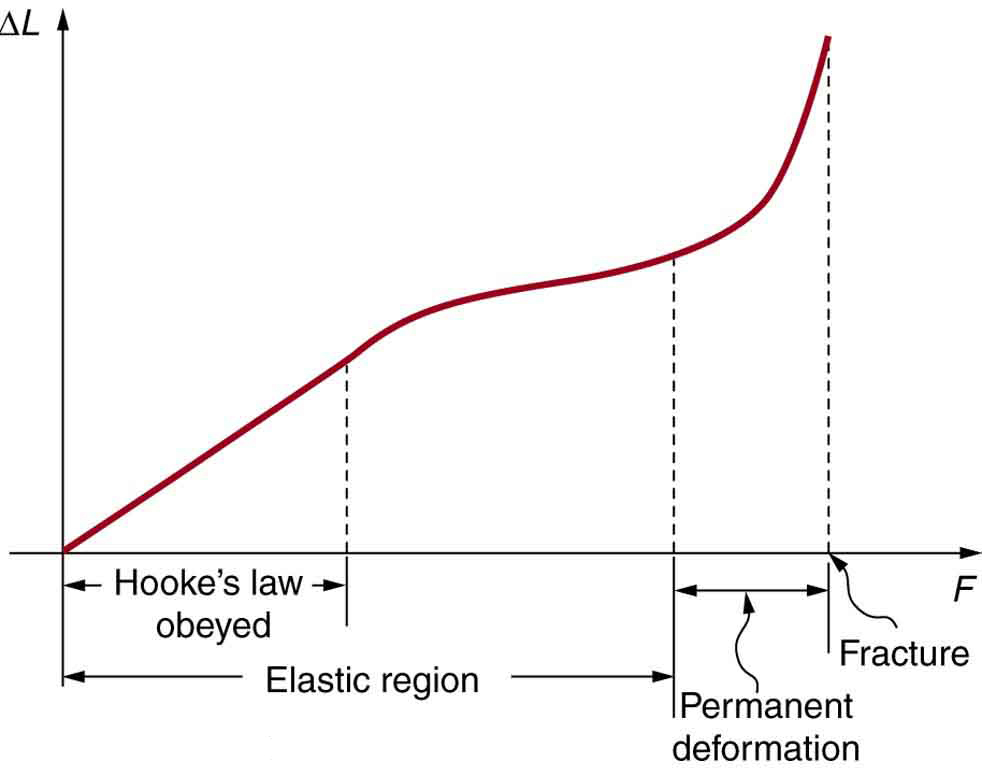
\includegraphics[width=0.48\textwidth]{../diagrams/rubber.jpeg}
  \end{center}
  \caption{\textbf{The stress-strain curve for rubber. Image courtesy of~\cite{rubr}.}}
\label{fig:rubber}
\end{wrapfigure}

An equally promising development in the field of epithelial tissue imaging is the work being done in the surface reconstruction of \emph{Drosophila} wings. Several softwares exist which can reconstruct a mesh of epithelial cells from an input image, but the most recent software released by L. Bai is able to take sets of images and faithfully reconstruct the apical face of a sheet of wing cells~\cite{3dwing}, even detecting 3d deformations. These imaging softwares will provide immense amounts of data about epithelial cell shapes and topology which will guide the development of future models, and perhaps serve as initial conditions and benchmarks for existing models. Unfortunately, the source code for the 3d imaging software is not freely available, and the possibility of developing an open source version ought to be considered. Very little is known about the accuracy of these softwares, as information about them comes exclusively from academic journal articles, and, depending on the quality of these imaging packages, competitive programs may be able to be developed in a short amount of time thanks to advanced libraries like Python's OpenCV~\cite{OpenCV}.

\section{Further Parallelization}
While the preceding ideas are very interesting and would contribute new ideas to the world of epithelial tissue modeling, the project of recreating the Honda-Nagai model was originally undertaken in the hopes of parallelizing the vast majority of the computations. Unfortunately, the trouble of efficiently storing a large tissue rendered the implementation of a parallel integrator seemingly impossible. 

The Chaste software is able to perform some computations in parallel, but only on the scale of a multi-core CPU, and not yet on the scale of a CUDA GPU~\cite{ChasteTutorial}. It is still possible to make a great contribution to the epithelial tissue community by discovering and sharing an effient datastructure and set of algorithms for storing and moving a sheet of epithelial cell vertices in parallel.

The first task in fully parallelizing the \emph{Epithelium}'s numerical integrations is storing the data in C arrays instead of classes, which will inevitably make the code's workings much more subtle than they currently are. Then, the next objective will be situating the data in an array in such that processors can effectively grab coalesced data chunks without too many expensive memory transactions. 

\section{Voronoi Tesselations}
The Honda-Nagai model \footnote{And other programs. The Voronoi Tesselation is one of the most famous algorithms in all of computational geometry. For more information see~\cite{tessel}} uses a periodic Voronoi Tesselation as the initial condition for the tissue~\cite{HondaNagai}, yet to the best of our knowledge an open source periodic Voronoi Tesselation program is unavailable. Indeed, the Voronoi Tesselation provides an ideal artificial initial mesh for an epithelial tissue simulation since all vertices have degree three and a careful choice of generating points can give all cells similar areas and perimeters. Several sources offer reliable software which computes a Voronoi Tesselation on the unbounded plane~\cite{boost, triangle}, while another freely available code performs the Voronoi Tesselation on 3D surfaces~\cite{voro++}, but none of these codes can perform the tesselation in a bounded box, or with periodic boundary conditions. 

The C++ Boost Library is a popular, heavily tested library for the C++ language, yet the Boost Voronoi Tesselation only computes the unbounded Voronoi Tesselation of a set of points, despite demand for a bounded Voronoi Tesselation as evidenced by questions~\cite{q1} on the programming website StackOverflow, and by the needs of epithelial modeling software. The lowest hanging fruit in the field of Voronoi Tesselations is the design of a bounding box algorithm for the Boost Voronoi Tesselation. A good second project would be to modify the Boost Voronoi functions so that they are able to produce periodic meshes. The expansion of this library would be a good service to modelers and to the C++ community in general.

\section{Visualization Software }
A final suggestion for the improvement of \emph{Epithelium}, and data presentation in general, is the development of an easy to use mesh visualization software which will take in data in a format similar to the OFF file format, and output an image of a mesh with highly customizable appearance. The vast majority of epithelial tissue simulations have rather bland graphical output, while others are very sharp and highly customizable. For examples of the current state of tissue visualization, see Figure~\ref{fig:fourgraphs}. 

